\documentclass[aspectratio=169]{beamer}

\usepackage{polyglossia}
\usepackage{csquotes}
\usepackage{libertine}
\usepackage[libertine]{newtxmath}
\usepackage{biblatex}

\setdefaultlanguage{czech}
\usetheme[progressbar=foot]{metropolis}

\definecolor{ctu}{HTML}{0072c6}
\definecolor{ctufit}{HTML}{f0ab00}

\setbeamercolor*{alerted text}{fg=ctu}
\setbeamercolor*{structure}{bg=white,fg=ctu}
\setbeamercolor*{palette primary}{use=structure,fg=white,bg=structure.fg}
\setbeamercolor*{palette tertiary}{use=structure,fg=white,bg=ctufit}
\setbeamercolor*{palette quaternary}{fg=white,bg=black}
\setbeamercolor*{progress bar}{fg=ctufit}

\makeatletter
\setlength{\metropolis@titleseparator@linewidth}{2pt}
\setlength{\metropolis@progressonsectionpage@linewidth}{2pt}
\setlength{\metropolis@progressinheadfoot@linewidth}{2pt}
\makeatother

\title{Implementace B-stromů na GPU}
\author{Duong Tat Dat, vedoucí: Ing. Tomáš Obenhuber, Ph.D.}
\institute{České vysoké učení technické v Praze, Fakulta informačních technologií}
\date{\today}

\begin{document}

\titlegraphic{
  \vspace*{0.25em}
  \includegraphics[width=0.25\textwidth]{images/fit-cvut-logo-cz}
}

{
  \metroset{progressbar=none}
  \begin{frame}
    \vspace*{2.25em}
    \titlepage
  \end{frame}
}

\begin{frame}
  \frametitle{Motivace}
  \begin{itemize}
    \item Grafické karty jsou mnohem výkonnější
    \item Poskrovnu datových struktur pro GPU
  \end{itemize}
\end{frame}

\begin{frame}
  \frametitle{Cíle}
  \begin{itemize}
    \item Představit implementaci B-stromů
    \item TODO: přidat vtipnou ukázku git commitu
  \end{itemize}
\end{frame}

\begin{frame}
  \frametitle{B-stromy}
  \begin{itemize}
    \item Specialization of $(a,b)$-tree
    \item Použita v databázích, souborových systémech
    \item Great for storing large amount of data
  \end{itemize}
\end{frame}

\begin{frame}
  \frametitle{CUDA}
  \begin{figure}
    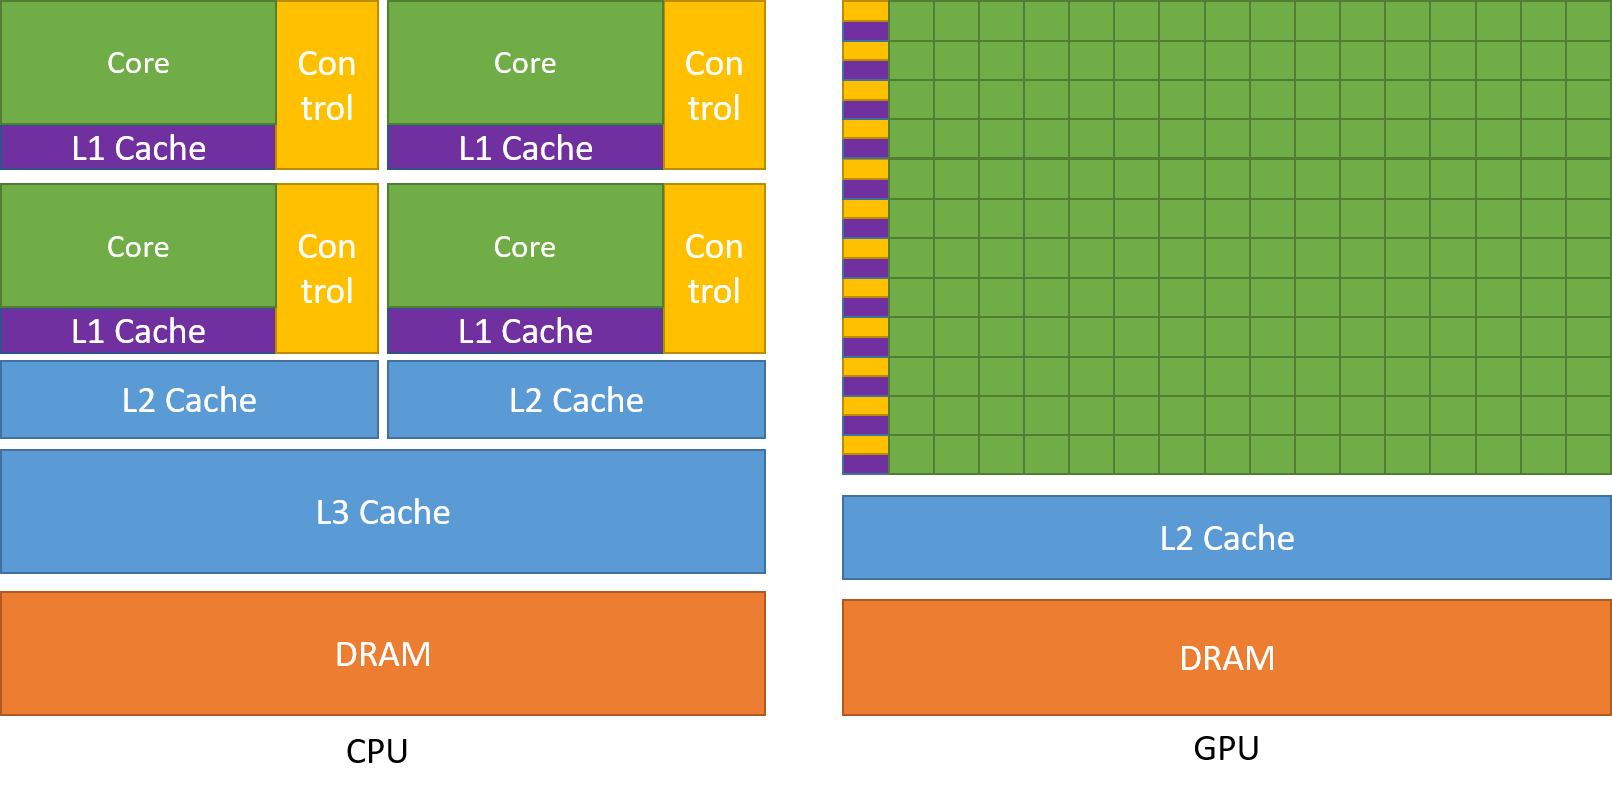
\includegraphics[width=0.8\textwidth]{components/figure/cpu-vs-gpu.png}
    \caption{Rozdíl mezi CPU a GPU}
  \end{figure}
\end{frame}

\begin{frame}
  \frametitle{Řešení}
  \begin{itemize}
    \item B+Tree
    \item Warp Cooperative Work Sharing
    \item B-Link-Tree
    \item
  \end{itemize}
\end{frame}

\begin{frame}
  \frametitle{Závěr}
  \begin{itemize}
    \item 15x až 30x rychlejší operace při vkládání a načítání dat
    \item Debugovací nástroj
    \item Du budoucna: srovnat se state-of-art
  \end{itemize}
\end{frame}

{
  \begin{frame}[noframenumbering,plain,standout]
    \LARGE{Děkuji za pozornost.}
  \end{frame}
}

\end{document}